\documentclass[12pt,a4paper]{article}

% ==================== 中文支持 ====================
\usepackage[UTF8]{ctex}

% ==================== 页面布局 ====================
\usepackage[margin=1in]{geometry}
\usepackage{setspace}
\onehalfspacing

% ==================== 数学与算法 ====================
\usepackage{amsmath,amssymb,amsthm}
\usepackage{mathtools}
\usepackage{algorithm}
\usepackage{algpseudocode}

% ==================== 图表 ====================
\usepackage{graphicx}
\usepackage{float}
\usepackage[font=small,labelfont=bf]{caption}
\usepackage{subcaption}

% ==================== 引用与超链接 ====================
\usepackage{hyperref}
\usepackage[style=gb7714-2015,backend=biber]{biblatex}
\addbibresource{references/bibliography.bib}

% ==================== 其他 ====================
\usepackage{enumitem}
\usepackage{booktabs}
\usepackage{xcolor}

% ==================== 定理环境 ====================
\newtheorem{theorem}{定理}[section]
\newtheorem{lemma}[theorem]{引理}
\newtheorem{corollary}[theorem]{推论}
\newtheorem{definition}[theorem]{定义}

% ==================== 标题信息 ====================
\title{\textbf{论文 Review：Optimal Resizable Arrays}}
\author{万宇（241880496）}
\date{2026年7月11日}

\begin{document}

\maketitle

\begin{center}
\begin{tabular}{ll}
\textbf{论文标题} & Optimal Resizable Arrays \\
\textbf{作者}     & Robert E. Tarjan, Uri Zwick \\
\textbf{发表信息} & SOSA 2023 (Symposium on Simplicity in Algorithms), 2023 \\
\textbf{Review 作者} & 万宇（241880496） \\
\textbf{日期}     & 2026-07-11 \\
\end{tabular}
\end{center}

\tableofcontents
\newpage

% ==================== 1. 引言 ====================
\section{引言}

对 Optimal Resizable Arrays 这篇文章做阅读理解同时补齐需要的知识。

% （待撰写）

% ==================== 2. 问题背景 ====================
\section{基础知识}
O代表上界,Ω代表下界.\\
均摊分析是用来分析某一特定操作的开销的分析方法，比如分析数组插入元素带来的开销。\\
均摊分析有聚合分析、记账分析、势能分析三种。\\
聚合分析就是先把所有操作的开销加起来然后求平均。\\
记账分析是一种简化版的势能分析，假设某一动作自身消耗为n，算的时候假设是m+n，即留m给别人，最后看m是多还是少还是刚好，调整m即可\\
势能分析类似于中学物理学的势能和动能，就是说在考虑一个操作的时候不能只看它自己的开销还要关注它对之后操作的开销的影响。\\
举个例子，假设一个vector采用超容则乘2复制的方法。那一个超容的插入的开销是O(n)，但它同时也便利了之后几次插入操作，因为它们不必再重复扩容和复制的过程了。\\
这就好比小球沿着非光滑曲面冲上高处，消耗动能产生摩擦热同时储存重力势能。\\
堆栈操作是一个很好的均摊分析的例子。\\
假设一个栈s支持三种操作，开销如下：\\
push:O(1);
pop:O(1);
pop\_k: $O(\min(s.size(),k))$;

聚合分析：\\
n次push：O（n）\\
所有pop:O(n)\\
平均：O(1)\\
记账分析：\\
每一次push设代价为2，留1\\
正好与pop抵消,故为O(1)\\
势能分析：\\
设一个势能函数Φ(s)=s.size()，即将元素的数目看作资源\\
则push资源增加，开销为2\\
pop资源减少，开销为0\\
故为O(1)\\
\section{这篇文章讲了什么？}
一共就讲了两个重点：一是在给定的条件下给出了一种数组的实现，使得访问代价为O(1)且空间为$N+O(N^{1/r})$，这是他们的核心结论，比之前的同方向的研究更好。
另一个是给定一个下界，说明你不可能做到一个数组的实现：在保持空间 $N+O(N^{1/r})$ 的同时还指望 grow 的时间小于 $\Omega(r)$，也就是让其他人别再试图往那个方向钻了。
\section{这篇文章的分层}
\begin{itemize}[left=0pt]
    \item 第一节：Introduction
    \item 第二节：问题定义
    \item 第三节：讲述前人的工作
    \item 第四节：关于一个有用的 lower bound
    \item 第五节：描述 $r=3$ 时的 resize 和 store 开销
    \item 第六节：扩展至任意 $r\ge2$ 的情况
    \item 第七节：对第六节中的方法的一个小瑕疵进行优化
    \item 第八节：提出抽象增长游戏（一个抽象的数学模型）
    \item 第九节：用抽象增长游戏证明在空间为 $N+O(N^{1/r})$ 时他们的实现是最优的
\end{itemize}

接下来的 review 我会按照原文的结构分成四个部分：

背景和铺垫：1--4

提出新方法：5--7

证明无法更牛逼：8--9

我自己的一些思考
\section{背景和铺垫}

\subsection{问题定义}
这篇文章讨论的问题不包括在arrary中间加或改元素的情况。\\
他们还假设了他们的系统里可以使用类似于free和malloc这样的工具来分配和释放任意位置和大小的空间且这种操作对每个单位的代价是常数级的。
也就是说，他们不管内存管理系统的实现，默认它已经足够好了。
然后他们介绍了一种叫做block的东西，他们令一个可变数组由若干定长数组的组合来实现的。这篇文章讨论的所有数据结构本质上都是blocks。
这是一个值得注意的地方，因为所有主流编程语言的可变数组都是由连续内存空间来实现的而不是用所谓的block。实际上我之前从来没听过block这种设计。
block一共可分为三种：数据block：直接存目标数据，索引block：存指向其它block的指针和辅助(auxiliary)block:存一些别的。这有点类似于操作系统中的分页内存管理机制中的页表和数据块和辅助位。\\
而这种分类是何意味呢？这主要是为了引出他们自己给出的一个丈量即：Definition  2.1$((s(N),t(N))$-implementation).Let $s(N),t(N)$ be  two  non-decreasing  functions.A  resizable  array  data  structure  is  said  to  be  
an$(s(N),t(N))$-implementation  if  it  uses  at  most  $N+s(N)$space to store an array of size N, and at most $N+t(N)$ space during a grow or shrinkoperation on an array of sizeN.
这个定义几乎贯穿全文也是本文最大的创新。即将一个可变数组的空间消耗分两种情况来看一种是增或减时的开销以及其它时候的开销。也就是他们敏锐的捕捉到了一个可变数组的开销不是一成不变的，这里面有可以操作的空间。而之前的所有研究者都没有抓住这一点。
\subsection{对前人工作的引用和论述}
\subsubsection{Two basic data structure}
一共讲了两种基本的数据结构，第一种是最蠢的，用一个N空间的定长数组来模拟一个可变数组，每一次删除或增加元素都要重新分配空间然后完成复制。这几乎没有意义，作者写它估计是为了水字数。
第二种是用的最广的即 geometric expansion /shrinking 结构，就是我们最熟悉的C++的vector的实现。均摊分析算下来grow 的代价为(1+1/a),shrink的代价为(1/a)。
这个结构已经不错了，也非常practical。
\subsubsection{The data structure of Sitarski}

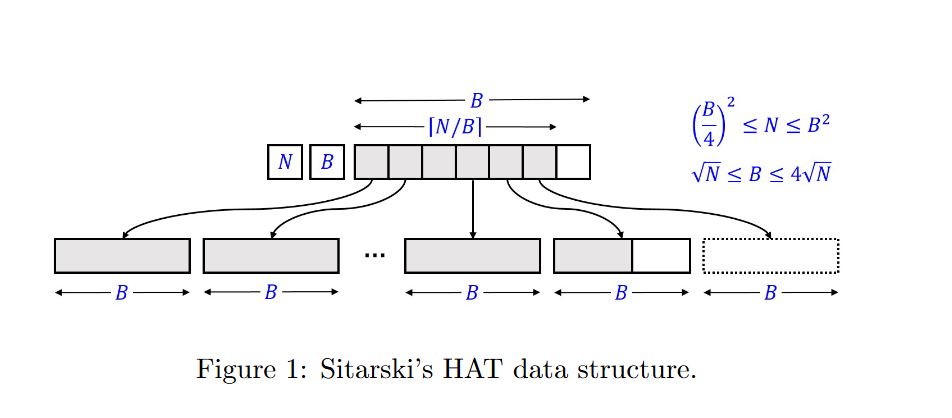
\includegraphics[width=1.0\textwidth]{Sitarski.png}
Sitarski的实现名字叫hashed array tree(HAT)。名字很高级但实际上既没有哈希也没有树。
它本质上就是数组套数组，还是页表那一套。它就是把一个数组切成小块每一个block大小为B，然后再来一个索引块，也为B，所有块大小都是B。
找元素的时候就查两次数组就好了。它的优势在于每次超容的时候只要加一个索引指向一直被维护的空数据block即可。
但其实它复杂度和geometric差不多。总的来说这还是一种很简单的很容易想到的实现。
下一个实现就是它的变形。
\subsubsection{The data structures of Brodnik et al.}
这个比较有意思，这个实现的美妙之处是 no rebuild is necessary and data items do not need moving。
它的实现思路和上一个类似。都是先查指针再插数据块。但不同之处在于每个数据块大小不一且呈现递增趋势。
之前Sitarski的做法的缺点在于当N越来越大，B由于要满足单次查询O(1)的条件而不得不扩大，这一扩大，就要重建和搬元素。
但是Brodnik的做法却不同，由于B自动增大，假设按1,2,3,4,.......n这个顺序来,最后的B和N的关系刚好是$B=\sqrt{2N}$。
但复杂度和前两种差不多，依旧是$N+O(\sqrt{N})$。
作者之后拿这个算法开刀来展开他的理论\\
\subsection{The lower bound of Brodnik et al. and its extension}
前面已经引出了Brodnik的实现，接下来提出了三个结论如下：
\begin{theorem}
Any data structure for maintaining a resizable array must at certain times use $N+\Omega(\sqrt{N})$ space, where $N$ is the current length of the array, even if only grow and access operations are performed.
\end{theorem}
\begin{theorem}
Any $(s(N),t(N))$-implementation of resizable arrays must have $s(N) \cdot t(N) \ge N$, even if only grow and access operations are supported.
\end{theorem}
\begin{theorem}
For any integer $r \ge 1$, any data structure that uses only $N+O(N^{1/r})$ space for storing a resizable array of size $N$ must occasionally use $N+\Omega(N^{1-1/r})$ space during a grow operation, even if only grow and access operations are performed.
\end{theorem}
我来展开说明。\\
首先，需要注意，这里所有的结论都是针对Brodnik的实现。有一个关键点在于这种实现下,Block的大小是递增的。\\
\begin{enumerate}
    \item Theorem 4.1 说明：这个定理是说一个数组在扩容的时候，总有那么一个时刻，假设这个时刻它的元素的数目为 $N$，那么此时它所需要的空间为 $N+\Omega(\sqrt{N})$。
    证明也很简单，显然随着N：数组元素的增加，k:索引Block的数量的增加是跳跃式的，即一个数组可能在两个时刻k相同但是Block的数目差距很大。
    显然所有的数据块都是必须的，这一部分开销为N，而索引块的容量比较复杂，因为是跳跃性的增加的。所以分类讨论。
    当k$\ge\sqrt{N}$时，空间消耗为$N+\Omega(\sqrt{N})$。
    但这只是极少数情况时k的取值，实际上k常常小于$\sqrt{N}$因为现有的索引块指向的数据块不被装满才是常态。
    当k小于$\sqrt{N}$时,平均下来每个数据块的大小必然大于$\sqrt{N}$，根据鸽巢原理，必然存在一个数据块，它的大小大于$\sqrt{N}$。
    回看这个大的数据块刚刚被分配的时候也就是它里面还是空的时候，假设此时数据块的总容量为$N'$显然此时的空间消耗为$N'+\Omega(\sqrt{N'})$（这里我们甚至没考虑指针的开销）。
    证明完毕。
    \item Theorem 4.2 说明：这个的证明其实和上面的4.1类似。首先重申一遍$s(N)$和$t(N)$的定义。$s(N)$表示在
    任何时候存储一个大小为$N$的可变数组所需的最多空间，$t(N)$表示在增长或缩小操作期间使用的最多空间。
    我们依旧只讨论除存数据的空间以外的开销。\\
    只要关注索引块和数据块和空白块的相对变化就好了。当空白块为空的时候所有的额外开销都用于储存索引，此时索引的数量就是$s(N)$(有个前提，索引项的大小是一个字，而以上我们所有的讨论都是以字为单位，忘了说了哈哈)。
    那么根据鸽巢原理，必然存在一个数据块，它的大小$\ge\frac{N}{s(N)}$。那么我们再回到这个大块被创建的时候还是空的时候，设此时的元素数目为$N'$，显然此时的开销为$N'+\frac{N}{s(N)}+else$。
    所以$t(N')\ge \frac{N}{s(N)}$，回到元素数目为$N$的时候，由于$t(N) \ge t(N')$，所以$t(N) \ge \frac{N}{s(N)}$。
    所以$s(N) \cdot t(N) \ge N$。
    证毕。\\
    注意，这个约束非常重要，因为无论层数r为多少，这个定理都成立，之后会反复用到。
    \item Corollary 4.3 说明：这就是从上一个结论导出来的必然结果，$\frac{1}{r}$只是一个人为选定的参数，不用纠结。\\
\end{enumerate}
\subsection{新方法的提出}
\subsubsection{一个简单的\texorpdfstring{$(O(N^{\frac{1}{3}}),O(N^{\frac{2}{3}}))$}{(O(N\^{}1/3), O(N\^{}2/3))}的实现}
这是一个承上其下的部分，通过之前的介绍，作者提出了一个简单的实现，满足空间为$N+O(N^{1/3})$，增长操作的开销为$O(N^{2/3})$。\\
这个实现的思路是这样的：\\
既然要实现s(N)为$O(N^{1/3})$，那么索引块的数量就必须是$O(N^{1/3})$，那么每个数据块的大小就必须是$O(N^{2/3})$。
我们考虑沿用之前提到的HAT的实现思路，即索引块指向数据块的一层查找。
但是问题很快出现了，依旧考虑数据块刚被分出来的时候，因为它的大小为$N^{\frac{2}{3}}$。
显然此时光是这一块的浪费了的开销为$N^{\frac{2}{3}}$，这就不满足$t(N)$为$O(N^{1/3})$的要求了。但是要满足{$(O(N^{\frac{1}{3}}),O(N^{\frac{2}{3}}))$}这个实现，索引块的数量又不能太大。
直接一根筋变两头堵了。\\
作者的解决方案是引入辅助块或者说缓冲块的方法。\\
也就是说，大体上还是延续之前的HAT的实现思路，但是对于最后分配的那一个内存块，我们不直接把它分配为一个数据块，而是先分配为一个辅助块（它能储存的元素数目上界为$N^{\frac{2}{3}}$），等到这个辅助块被填满了之后再把它转化为一个数据块。
而这个辅助块用经典的r=2的HAT来实现。用页表来类比（即B的大小为$N^{\frac{1}{3}}$），就是一个混合页表。\\
因为不直接存储一个大的数据块而是内部维护一个容量缓慢增大的辅助块，所以在这个辅助块被填满之前，空间开销是非常小的。额外的开销控制在$\Omega(N^{1/3})$。\\
至此，我们就达成了我们的目标。
\subsubsection{一个\texorpdfstring{$(O(rN^{\frac{1}{r}}),O(N^{1-\frac{1}{r}}))$}的实现的优化}
从前一小节中我们已经能看出，只要$r\ge2$，我们就能实现一个$(O(N^{\frac{1}{r}}),O(N^{1-\frac{1}{r}}))$的实现。就好像多级页表一样，我们完全可以数组里面套数组来实现空间的高效利用。
但这种递归的实现方式太过复杂了，假如说r=5，那层数就太多了，作者提出了一个优化的实现。它在空间复杂度上等价（之后会说明这一点）但它是扁平的，易于理解的。\\
简单来说，在递归的实现方式下不是存在一个块的大小和容量的平方关系吗，那就直接分配块的时候就按照这个来就好了。这样就不用查来查去了（怎么有种伙伴系统的感觉，只不过伙伴系统里面是2的幂这里是B的幂）。\\
具体实现见下图：\\
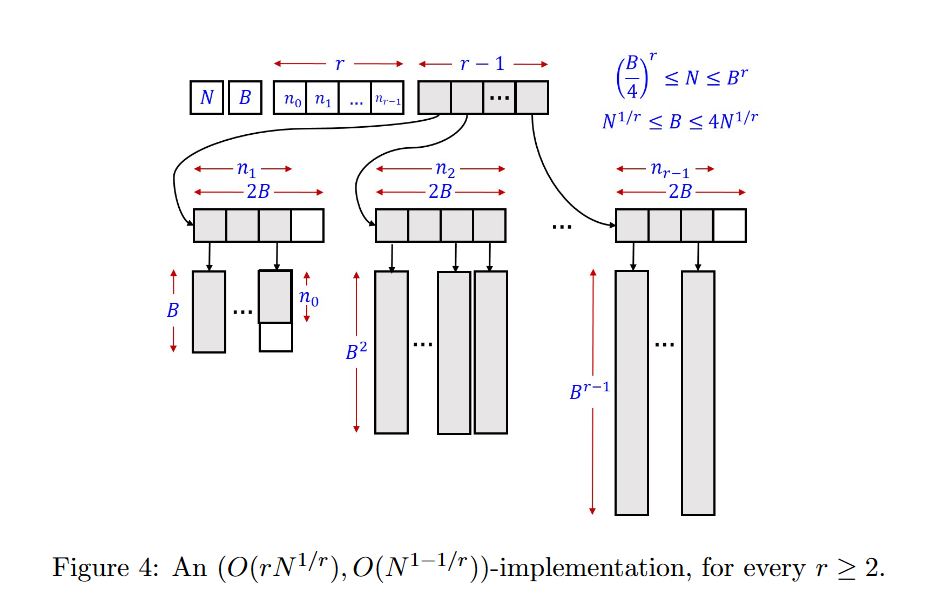
\includegraphics{rN.png}
这种扁平化的实现方式的好处是它的层数只有两层，索引块和数据块故你想要访问任何一个数据块的时间开销都是$O(r)$。并且它的空间复杂度和之前的递归实现方式是等价的。\\
对这种数据结构进行元素的删或增是非常容易的，只需要记录当前有哪些大小的块和各个大小的块的数目就好了。如果操作是增，且目前没有空位则先检查合并可能，倘若元素块已经可以向上合成了（用一个位图来表示就是  2B-12B-12B-12B-12B-12B-1，只要最后一位是2B-1即可，至于为什么不是B-1，这是一个小巧思）,
那这种情况直接向上合成到不能合成再分配小块即可。否则直接分配就好了。删的操作就是反过来，只是将检测是否可合并改为是否需要拆分。\\
然后下面我给出这种思想的伪代码实现(核心意思就是我这里说的):\\
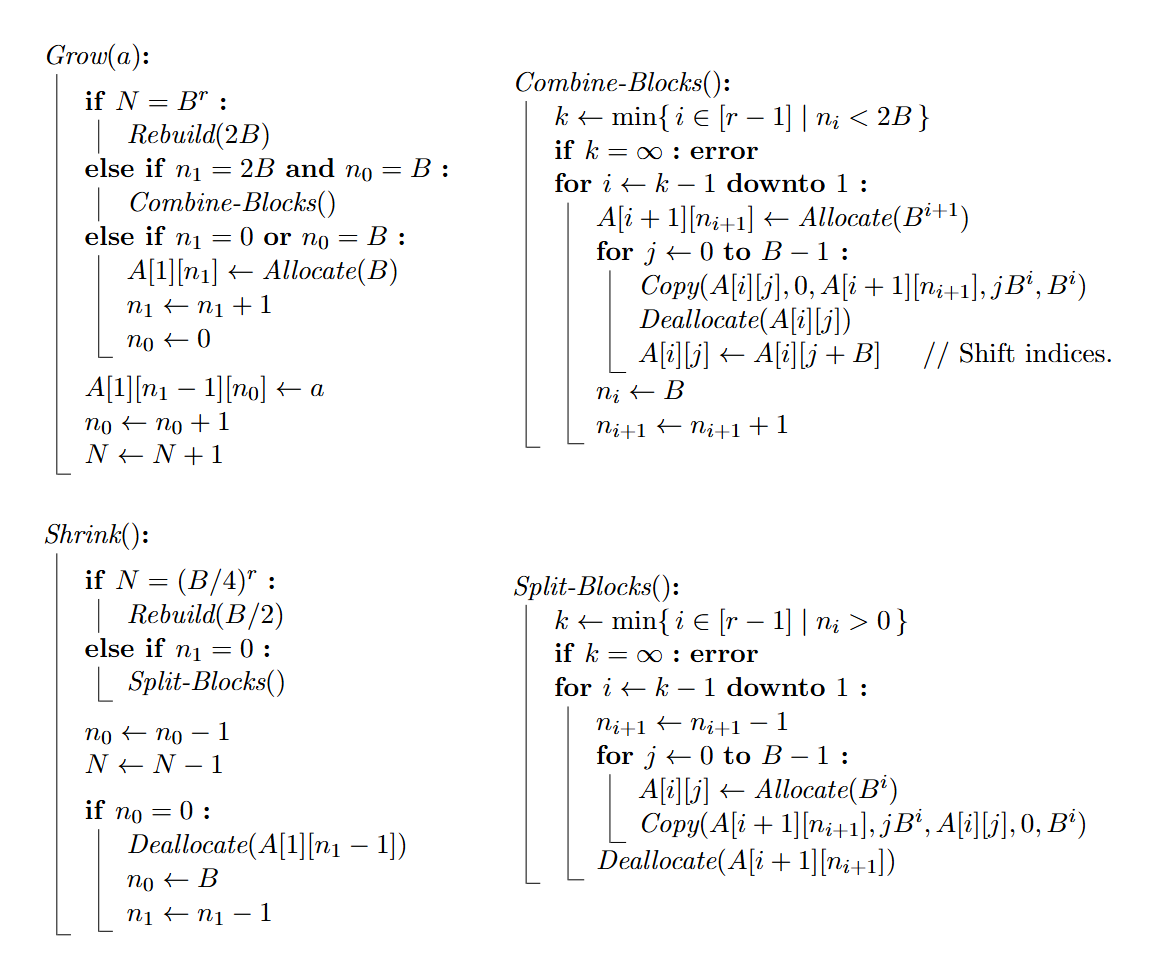
\includegraphics[width=0.8\textwidth]{fakenode.png}
接下来看看Grow和Shrink操作的时间复杂度的均摊分析。
因为这是一个涉及到空间扩充的操作，所以直接用记账分析就好了。
这里原文讲了三页纸但其实很简单。\\
首先我们需要一点直觉即这种数据结构的开销必然和它的层数r挂钩，因为你r越多，分出的块就越多，需要转表的次数也就越多(这一点在之前提到的递归的实现里反而体现的更明显，这里扁平化了其实不太好看)。\\
所以我们可以假设每次操作的开销为$O(r)$，但这个账显然不是平均分布的，那些越小的子块变动的越频繁，因为它们容量小，它们更容易发生扩容和合并给它们记r。而那些最大的块里的元素，它们从被创建开始就没动过。所以直接给它们记0，设层数为i，发的账为r-i。
我们接下来只讨论合并的操作的开销就好，因为单纯的增加元素开销就是O(1)而且只用做一次。而没一次下层的元素往上移动就是用上层的空间中复制下层的元素来实现的，所以每一个元素向上跃迁一次，开销就是O(1)\\
如果一个块的大小为$B^{k}$也就是说它是由大小为B、$B^{2}$、$B^{3}$、...、$B^{k-1}$的块合并而成的，那么它的开销就是$B\times (B+B^{2}+B^{3}+...+B^{k-1})\le2B^{k}$\\
而之前我们给每一个元素发了(r-i)的账，i是它所在的块的层数。第i层的块的大小为$B^{i}$，所以每一个元素的账为$r-i$，而每一个块的大小为$B^{i}$，所以每一个块的账为$B^{i}\times (r-i)$而从第i层到k层消耗的账为$B^{i}\times (i-k)$\\
每一层的消耗的账为$B^{i}\times (r-i)$，而从第i层到k层消耗的账为$B^{i}\times (i-k)$刚好相等。（也可以加起来求平均，是一个等差数列乘以等比数列的形式，可以求和）。
所以每一个元素的账都足够支付它的开销。\\
所以Grow的均摊开销为$O(r)$。
Shrink同理。\\
同时作者还有一个小巧思，就是冗余加速。比方说1999+1这个运算，正常来说要进位3次。但作者可以允许冗余，即只有一位等于20的时候才进位，这样就极大的减少了进位的次数，也就减少了内存块复制的次数。
而为了进一步减少级联的进位操作还规定一次运算只能发生一次进位，倘若本次运算没有触发抵达2B则扫描高位是否溢出，溢出则处理。
不难看出在这种情况下每一次加法最多带来两次位的变化，所以开销直接变成$O(1)$。
\subsubsection{访问加速}
这里说白了就是经典的位运算加速访问。之前的老访问方式是用多级页表的方式去一次次的查表，显然这种方式对页表这种地址缺乏规律的情况是最好的但目前这种分块有一个很重要的东西是块的大小是B的幂。
直接把要找的元素的索引和目前元素的总数转为B进制数。假如目标元素总数为N此时的B为8，转为$N_B$后为(1,2,3,4,5,6,7)而索引转换后为(1,2,3,3,1,1,1,)，那么就应该去第四位找那个元素。
但这种情况成立不代表永远成立，因为我们的表示是冗余的而之前的表示方法都是传统的转化为B进制，这种方法无法正确反映每一个size的内存块的数量。所以要采用补救措施。\\
比方说B=5时$N_B$为(1,0,3,1)(位数左低右高)，$S_B$为(0,3,2,1)。从高到低比发现第二位首次出现小于关系，如果数据的实际存储就是按照标准的B进制来，那这里就可以结束了，但实际
存储为冗余存储因为要保证grow的速度（见前文）。这里发现是落在2号块里，最理想的情况是索引刚好位于1号块的和与二号块和一号块的和之间，这样就能一步到位因为此时有没有冗余都一样，直接就能判断去哪里找元素。
但此时一号块的和只有125，不满足，所以要打补丁。先看上帝视角，$N_B$=(6,9,6,0)，$S_B$=(5,7,6,0)，显然在第1号位。但是这个转换在计算机里太复杂了，不可能每次打补丁都要这么做。所以要做差。
注意这里有一个前提就是每一位是否存在冗余，数据结构都是维护了的。所以因为差是15而二号位的上一位也就是一号位没有发生冗余故容量为20，装下了，所以在一号块里。\\
综上，通过这种方式，成功实现了访问加速，现在的访问速度直接到了$O(1)$。
\subsubsection{进一步空间优化：去除r这个小瑕疵}
之前给出了一个$(O(rN^{\frac{1}{r}}),O(N^{1-\frac{1}{r}}))$的实现都是基于r为一个固定的常数的。在这种情况下，我们已经论证了它就是最优的。但是实际上，r可以是一个随着N变化而变化的值。直觉就是随着N的增大，原有的层数太少了，因为当B给定的情况下
如果r给定，N就定了，所以如果当前的r容不下N，那N就要变化，所以显然存在一个N到r的映射。因为这是一个等比数列和的关系，所以r=r(N)=$O(\log N)$当然这只是便于理解，不然这个r一直出现会把人搞蒙。
接下来我们在这个语境下讨论将存储时所需的空间进行优化。\\
从静态和动态入手。
首先我们要建立一种直觉，一个数据结构要被存储，它大多数时候都是静态的，此时它的空间消耗为$N+s(N)$，但是当你需要进行增和删的时候，就需要开辟一个临时空间并进行元素的复制。
显然，这个临时空间越大，需要的$t(N)$也就越大。但是这个数组大部分时候都是静态的，只有当分配了新的块的时候它才需要考虑$t(N)$的开销。前文提到过$s(N)\cdot t(N)\ge N $，说明它们之间存在
某种此消彼长的关系，那么我们是否可以以$s(N)$小幅上涨为代价让$t(N)$降下来？这是可行的，实际上可以将
$(s(N),O(N))$的实现转化为$(s(N)+O(\frac{N}{t(N)}),s(N)+O(t(N)))$的实现，只要内存分配方式是一次分配一次到位并清空旧空间。（这个条件很常见，不用在意）
接下来我来证明它：\\
这不是严格的那种数学证明实际上也不需要这么做，因为这里本质上是在讨论内存的分配方式而没有改变数据结构的底层逻辑，不同的分配方式带来不同的效用，根据前文提到的所有约束我们可以看出
这个实现是正确的因为它满足$s(N)\cdot t(N)\ge N$，也就是说确实存在这种实现。
我们只要找出这种数学上的模型的具体实例就能证明这是可行的了。还记得之前我们提到过对于一个$(O(N^{\frac{1}{3}}),O(N^{\frac{2}{3}}))$的讨论时为了让$s(N)$缩小到$O(N^{\frac{1}{3}})$时
做的工作吗？这里也是差不多的。我们发现，当一个resized array增长时，临时空间相对于当前的N的最大的时候就是当临时空间刚刚被分配的时候。此时，旧的待复制的内存块还在，而新的待
填充的内存块也在，这个瞬间，对空间的压力是最大的。所以我们要想方设法解决这个问题，即旧的和新的同时存在的问题，只要让新的空间被分配的同时复制一部分旧的元素同时释放掉一部分旧的空间就行了。
也就是不要一次性搬家，只要等新家的一个房间装修好了就可以从旧的家开始搬东西了。说白了就是新的块的粒度细一点，浪费的空间小一点。接下来我们假设某一时刻分配了一个块，它的大小大于$O(N^{1-\frac{1}{r}})$即大于t(N)。
(小于它的空间不用讨论，那可以接受).那就不要一次性分配这个块，而是分配$\frac{N}{t(N)}$个块按照$B,B^2,B^3.......$来分配空间就好了（B在此时的大小还是满足$ N^{\frac{1}{r}} ≤ B < 4N^{\frac{1}{r}}$），这就和之前提到的那个实现如出一辙。现在
我们知道了这种实现的过程峰值不可能大于$s(N)+O(t(N))$，因为一共就一个没装满的空间且它不可能大于$t(N)$。那为了维护这$\frac{N}{t(N)}$个块，就需要这么多个指针，所以永久存储就是
$s(N)+O(\frac{N}{t(N)})$这么多。所以对于
$(O(rN^{\frac{1}{r}}),O(N^{1-\frac{1}{r}}))$这个实现，我们带入进去就能把它变成$(O(rN^{\frac{1}{r}}),O(rN^{\frac{1}{r}}+N^{1-\frac{1}{r}}))$
这个式子很丑，引入一个不等式$r\le \frac{\log (N)}{2\log( \log N) }$这是一个对r的取值的约束。
然后就得到了一个漂亮的式子：$(O(rN^{\frac{1}{r}}),O(N^{1-\frac{1}{r}}))$\\
这个实现的访问开销均摊开销下来和前一个一样。都是$\Omega(r)$。\\
至此，这篇文章的第一个要点就将完了，就是反复的在临时和恒定里做文章。\\
\subsection{为何无法更牛逼}

\subsubsection{增长游戏}
增长游戏的篇幅很长，有6页都在讲这个玩意儿。但说白了，他就是对现有的数据结构做一个简化，之间不是贴了个伪代码吗？这个增长游戏就是把其它操作的开销删掉，只留下元素拷贝的开销。
因为作者想证明的是如果你只允许$ N + cN^{1/r}$ 的永久额外空间（即 $k ≈ cN^(1/r)$），那么均摊代价至少是 $\Omega(r)$。
所以如果在一个理想的模型里都没法超过这个下界，实际情况就更不可能了。我接下来简单讲讲我对增长游戏的理解。\\
用(N,k,l)来表示一个增长游戏。
N表示一共要填入N个元素，k表示一共有k个块可以被填入，每一个内存块都是一个数组，l表示一个有元素的数组中允许的未被利用空间的最大值。
显然，某个时刻最多只有一个arrary存在未被装满的情况。所以每个时刻额外开销最多k+l,k表示指针数目，l表示多余空间。
接下来我用伪代码展示增长游戏的所有规则。//
% ─── 全局状态 ───
\textbf{全局状态}
\begin{quote}
\begin{tabular}{@{}ll@{}}
$k$          & 子数组数量上限 \\
$\ell$       & 第一个非空子数组允许的空位数 \\
$N$          & 当前已插入元素总数 \\
$A[1\ldots k]$ & 每个子数组存储的元素个数（$0$ 表示空） \\
总代价       & $= 0$
\end{tabular}
\end{quote}

% ─── 主过程 ───
\begin{algorithm}[ht]
\caption{插入一个新元素：\texttt{Grow()}}
\label{alg:grow}
\begin{algorithmic}[1]
\Statex \qquad\textbf{── 情况一：第一个非空子数组还有空位 ──}
\State $i \gets \Call{FirstNonEmpty}{}$ \Comment{最小的满足 $A[i]>0$ 的 $i$}
\If{$i \neq \text{null} \land A[i] < \ell+1$}
    \State $A[i] \gets A[i] + 1$
    \State 总代价 $\gets$ 总代价 $+ 1$
    \State $N \gets N + 1$
    \State \Return{}
\EndIf

\Statex \qquad\textbf{── 情况二：全满但还有空子数组 ──}
\State $j \gets \Call{LastEmpty}{}$ \Comment{最大的满足 $A[j]=0$ 的 $j$}
\If{$j \neq \text{null}$}
    \State 分配新子数组，大小 $\gets \ell+1$
    \State $A[j] \gets 1$ \Comment{新元素放在第一个位置，剩 $\ell$ 个空位}
    \State 总代价 $\gets$ 总代价 $+ 1$
    \State $N \gets N + 1$
    \State \Return{}
\EndIf

\Statex \qquad\textbf{── 情况三：$k$ 个子数组全满 ──}
\State \Comment{玩家选择要合并多少个子数组}
\State $i \gets \Call{ChooseMerge}{}$ \Comment{玩家选择，$1 \le i \le k$}

\State $sum \gets 0$
\For{$m \gets 1$ \textbf{to} $i$}
    \State $sum \gets sum + A[m]$ \Comment{统计要拷贝的元素总数}
\EndFor

\State 分配新子数组，大小 $\gets (\ell+1) + sum$
\State 将 $A[i], A[i-1], \ldots, A[1]$ 的元素按顺序拷入新子数组
\State 将新元素放在新子数组的第一个空位上
\State 释放旧子数组 $A[1\ldots i]$

\State $A[i] \gets sum + 1$ \Comment{新子数组成为新的 $A[i]$}
\For{$m \gets 1$ \textbf{to} $i-1$}
    \State $A[m] \gets 0$ \Comment{前面的全部变空}
\EndFor

\State 总代价 $\gets$ 总代价 $+ 1 + sum$ \Comment{每个元素拷贝算一次}
\State $N \gets N + 1$
\end{algorithmic}
\end{algorithm}

% ─── 辅助函数 ───
\begin{algorithm}[ht]
\caption{辅助函数}
\label{alg:helpers}
\begin{algorithmic}[1]
\Function{FirstNonEmpty}{}
    \For{$i \gets 1$ \textbf{to} $k$}
        \If{$A[i] > 0$}
            \State \Return{$i$}
        \EndIf
    \EndFor
    \State \Return{$\text{null}$} \Comment{全空}
\EndFunction

\Statex

\Function{LastEmpty}{}
    \State $last \gets \text{null}$
    \For{$j \gets 1$ \textbf{to} $k$}
        \If{$A[j] = 0$}
            \State $last \gets j$
        \EndIf
    \EndFor
    \State \Return{$last$}
\EndFunction
\end{algorithmic}
\end{algorithm}

% ─── 关键点 ───
\textbf{关键点}
\begin{itemize}[nosep]
    \item 玩家只在\textbf{情况三}有选择权，其余两种情况是强制的可以视为系统自己操作。
    \item 代价 = \textbf{拷贝操作次数}。情况一和情况二是 $1$（只放一个元素），情况三是 $1 + {}$拷贝的元素总数。
    \item 空子数组必须在最前面这个约束，由合并操作自动保证（$A_1$ 到 $A_{i-1}$ 被清零，刚好成为空子数组的"前缀"）。
    \item $\ell = 0$ 时，每个非空子数组都是满的（大小 $=1$），情况一和情况二退化成同一种。
\end{itemize}
规则很简单，接下来用$C_{N,k,l}$表示最小总开销，$A_{N,k,l}$表示$\frac{C_{N,,k,l}}{N}$\\
我们开始寻找$A_{N,k,l}$。原文在这里讲了大半天，其实就四个要点。
一是定义状态，二是算精确表达式，三是算均摊下界，四是做扩展。\\
定义一个向量$a=(a_1,a_2,a_3,......,a_k)$，$a_i$
是子数组$A_i$当前装了多少元素。
由前文的定义可知，如果$a_i$为0，那么$a_i$到$a_{i-1}$全是0。
我们用$C(a)$来表示达到某个状态的最小消耗。
还有一个要点：$C_{N,k,l} = (l+1) \times C_{N/(l+1), k, 0}$

允许 l 个空位等于把 l+1 个元素打包成一个不可拆的块，所以只要分析 l=0 就行。
之后的大部分分析都默认l=0.



一个C包含了很多个子数组，我们要考虑它的代价只需要考虑所有子数组的代价和即可（注意A不能这么算）。
其实就是大问题拆成小问题的思想。\\
显然$C(a₁,...,aₖ) = C(0,...,0, aₖ) + C(a₁,...,aₖ₋₁)$


，从而$C(a₁,...,aₖ) = Σⱼ C(0,...,0, aⱼ)$。

我们再看块的聚合的那一步，即发生拷贝的时候。
$C(0,...,0, aₖ) = C_{aₖ-1, k} + aₖ$因为已经到了临界点了，这里必须分配一个$a_k$的空间。\\




合起来：$C(a) = N + Σ_{j=i}^{k} C_{aⱼ-1, j}$。

也就是说
总代价等于每个元素插入的 1 + 每个子数组的合并代价。
这样我们就找到了要达到某个状态的递归公式。
这对于我们寻找最终表达式很有帮助，因为我们只要知道任意一个$C_{aⱼ-1, j}$的真正表达式就能得出答案。\\
于是思考N 个元素分到 k 个槽，怎么分代价最小？如果某个槽元素太多，它迟早被合并，拷贝成本高。如果太分散，合并次数频繁。

最优状态必须让所有槽的"边际成本"相等。就像一个经济体里，资源要配置到边际收益相等时才效率最高，也就是说，每次装入一个元素
都要想想它给这整个结构带来了什么，它一方面完成了装入元素的任务令一方面也带来了未来拷贝的风险。
所以不可能一直往一个槽里装元素，因为装入之后该槽的价值就会降低。最理想的状态就是每个槽都均衡的下降。
逻辑上是这样的。
数学上，边际成本相等意味着：每个 aⱼ 必须落在一个狭窄区间内。这个区间恰好由二项式系数划定
$aⱼ ∈ [ C(n+j-2, j), C(n+j-1, j) ]$

其中 n 由 N 的位置唯一确定：$C(n+k-1,k)−1 ≤ N ≤ C(n+k,k)−1。$
以上是作者给出的结论，有点抽象，但是想清楚了就简单。\\
首先看两个数学公式：$$
\binom{n}{k} = \binom{n-1}{k-1} + \binom{n-1}{k}
\qquad
\sum_{i=0}^{k} \binom{n+i-1}{i} = \binom{n+k}{k}
$$
这是后面证明的基础。
我们还要引入一个数n，这是最最最核心的地方，因为如果只考虑N和k，我们就无法完成一个resizable arrary到增长游戏的抽象。
因为无法反映出B的大小和组织方式。
n可以视作向每个段中塞一个元素的代价同时也是槽的容量。其实只要将这一部分和之前讲的各种数据结构实现结合起来看就一目了然了。
n可以理解为B的大小。
注意，n是会随着N的变化而变化的。
从直觉上将，n与N和k之间一定存在某种关系。因为你要装的元素数目定了，允许的槽数定了，剩下没定的就是槽的大小了。
虽然对于游戏者而言，这个n是不可见的，但我们依旧需要这个n来做分析，这是很重要的地方。后面会说为什么一定要它。
但同时从另一个视角来看，$C(a) = N + Σ_{j=i}^{k} C_{aⱼ-1, j}$前面提到过这个公式。
我们可以手推这个公式，发现$C(a)$有一个特点，那就是它存在跳变。跳变当且仅当发生在发生合并时，n就是每一个段的编号。
而其它所有时候差分（插入一个元素的代价变化量）都是平滑的。所以我们就必须要思考突变的发生条件。\\
这就是前面那个结论的由来，用数学归纳法证明。\\
\paragraph{前置：归纳假设}

假设对更小的参数，定理已成立。也就是说，对 $(a_j-1,\,j)$ 这套更小的参数，存在唯一的 $n'$ 使得：

$$
\binom{n'+j-1}{j} - 1 \leq a_j-1 \leq \binom{n'+j}{j} - 1
$$

并且：

$$
C_{a_j-1,\,j} = a_j \cdot n' - \binom{n'+j}{j+1}
$$

\paragraph{第一步：确定 $n'$}

$a_j$ 被约束在最优区间内（由归纳假设的 (iii)）：

$$
a_j \in \bigl[\, \binom{n+j-2}{j},\; \binom{n+j-1}{j} \,\bigr]
$$

所以 $a_j-1$ 的范围是：

$$
\binom{n+j-2}{j} - 1 \leq a_j-1 \leq \binom{n+j-1}{j} - 1
$$

对比分段条件：

下界 $\binom{n+j-2}{j}-1$ 对应 $n'+j-1 = n+j-2$，即 $\mathbf{n' = n-1}$。

上界 $\binom{n+j-1}{j}-1$ 对应 $n'+j = n+j-1$，即 $\mathbf{n' = n-1}$。

所以整段内 $n' = n-1$。

\paragraph{第二步：代入递推}

把 $n' = n-1$ 代入归纳假设的公式：

$$
C_{a_j-1,\,j} = a_j \cdot (n-1) - \binom{n+j-1}{j+1}
$$

再代入递推公式 $C(a) = N + \sum_j C_{a_j-1,\,j}$：

$$
\begin{aligned}
C(a) &= N + \sum_j \left[ a_j(n-1) - \binom{n+j-1}{j+1} \right] \\
     &= N + (n-1)\sum_j a_j - \sum_j \binom{n+j-1}{j+1} \\
     &= N + (n-1)N - \sum_j \binom{n+j-1}{j+1} \\
     &= N \cdot n - \sum_{j=1}^{k} \binom{n+j-1}{j+1}
\end{aligned}
$$

\paragraph{第三步：曲棍球棒恒等式收尾}

令 $i = j+1$，则有：

$$
\sum_{j=1}^{k} \binom{n+j-1}{j+1}
= \sum_{i=2}^{k+1} \binom{n+i-2}{i}
$$

用曲棍球棒恒等式：

$$
\sum_{i=0}^{k+1} \binom{(n-2)+i}{i} = \binom{(n-2)+(k+1)+1}{k+1} = \binom{n+k}{k+1}
$$

从中减去 $i=0$ 和 $i=1$ 两项：

\begin{itemize}[nosep]
  \item $i=0$：$\binom{n-2}{0} = 1$
  \item $i=1$：$\binom{n-1}{1} = n-1$
\end{itemize}

所以：

$$
\sum_{j=1}^{k} \binom{n+j-1}{j+1}
= \binom{n+k}{k+1} - 1 - (n-1)
= \binom{n+k}{k+1} - n
$$

\paragraph{代回}

$$
\begin{aligned}
C(a) &= N \cdot n - \left[ \binom{n+k}{k+1} - n \right] \\
     &= N \cdot n - \binom{n+k}{k+1} + n \\
     &= (N+1)n - \binom{n+k}{k+1}
\end{aligned}
$$


至此，我们得出了精确公式，最难的地方结束了。\\
有了精确公式一切都好办了，接下来看看这个游戏开销的均摊下界。
边界情况 $N = C(n+k, k)-1$
$C_{N,k} = [kn/(k+1)] \times (N+1)$

所以均摊代价 $A_{N,k} = C_{N,k}/N ≥ k(n-1)/(k+1) ≥ (n-1)/2$。\\
水到渠成，
然后证明它是紧的。
我们发现$N=C(n+k,k)-1$时，算出来的均摊时$\frac{kn}{k+1}$，这和之前算的是一个量级。所以是可达到的所以是紧的。\\
但说老实话，我感觉这个取值像是天上掉下来的。可能是我理解不够深吧，反正是搞出来了。

最后来对现有的这个结论做一个扩展，目前它还是狭义的，因为之前定义增长游戏的时候就说了只允许一种合并：A₁ 到 Aᵢ（必须从最前面开始，连续一段）。
但真实数据结构的合并很灵活，如果不堵上这个骷髅人家就可以说你这个下界不严谨因为我可以通过合并的骚操作来绕开你的下界。
但堵上也不难，只要化规就好了。\\
考虑以下两种额外权利：允许合并中间连续段和允许合并任意子集。
所有合并方式都可以由这两种方式连带最初的方式来表达。\\
对于第一个用这种实现：选 1 ≤ i < j ≤ k，把 $Aᵢ, Aᵢ₊₁, ..., Aⱼ$ 合并到 Aⱼ 里。$A₁...Aᵢ₋₁$ 整体往右挪，前面腾出来的变空。不插新元素。代价 = 被合并的元素总数。
其实就是要看这个式子：$C(0,...,0,a_1,...,a_{i-1},\sum_{l=i}^{j}a_l,a_{j+1},...,a_k)$
拆成$C_{k-1}(0,...,0,a_1,...,a_{i-1})+C_k(0,...,0,\sum_{l=i}^{j}a_{l})$
前者不用管，都没动。
对于后者显然小于$C_k(0,...,0,a_i,...,a_{k-1})+\sum_{l=i}^{j}a_{l}$
所以这种合并的开销并没有变小。\\
第二种情况的证明方法一样，只不过是选任意子集 I =$ {i₁, ..., iᵣ} ⊆ [k]$（不要求连续），把 $A_{i₁}, ..., A_{iᵣ}$ 合并到 $A_{iᵣ}$ 里，外加一个新元素。I 之外的其他子数组不动。代价 = 被合并的元素总数 + 1。
放缩即可。\\
\subsubsection{确实无法更牛逼了}
直接把增长游戏的逻辑套到真实的数据结构中。$k = rN^(1/r)$（槽数 = 永久额外空间）
$l = rN^(1/r)$（空位数 = 冗余空间）
因为$C_{N, k, l} = (l+1) \times C_{N/(l+1), k, 0}$
然后来建立
n和r之间关系。
只要证明n和r是一个量级就好了，这样两边的结论就都能联通了。
假设n=$ar(a\le 1)$。
只要验证此时这个ar能够胜任n就行了。直接带前面的n的定义公式\\
$\binom{n+rN^{\frac{1}{r}-1}}{rN^{\frac{1}{r}}}$。
把上式用$C(n,k)\le (\frac{en}{k})^{k}$放缩一下，得到
$(\frac{e(a+1)N^{\frac{1}{r}}}{a})^{ar}$
之前说过，r大概是$\log N$这个量级的，取a=0.5发现此时这个项小于$N^{\frac{3}{4}}$
这个项还是比N小，说明最合适的a其实大于0.5。不过无关紧要了，得证。\\


\section{分工说明}

本项目所有工作由同一人独立完成。包括：

\begin{itemize}
    \item 论文选题与精读
    \item 文献检索与综述
    \item Review 正文撰写
    \item 个人反思写作
    \item 项目管理与版本控制
\end{itemize}

AI 工具（GitHub Copilot / ChatGPT 等）的使用记录见 \texttt{records/ai-usage.md}。

% ==================== 8. 参考文献 ====================
\section{参考文献}

详见 \texttt{references/bibliography.md}。

% （参考文献列表将在 bibliography.md 中维护）
% 如需使用 BibLaTeX，取消下一行注释：
% \printbibliography

\end{document}
